\documentclass[12pt]{extarticle}
%Some packages I commonly use.
\usepackage[english]{babel}
\usepackage{graphicx}
\usepackage{framed}
\usepackage[normalem]{ulem}
\usepackage{amsmath}
\usepackage{amsthm}
\usepackage{amssymb}
\usepackage{amsfonts}
\usepackage{enumerate}
\usepackage[utf8]{inputenc}
\usepackage[top=1 in,bottom=1in, left=1 in, right=1 in]{geometry}

%A bunch of definitions that make my life easier
\newcommand{\matlab}{{\sc Matlab} }
\newcommand{\cvec}[1]{{\mathbf #1}}
\newcommand{\rvec}[1]{\vec{\mathbf #1}}
\newcommand{\ihat}{\hat{\textbf{\i}}}
\newcommand{\jhat}{\hat{\textbf{\j}}}
\newcommand{\khat}{\hat{\textbf{k}}}
\newcommand{\minor}{{\rm minor}}
\newcommand{\trace}{{\rm trace}}
\newcommand{\spn}{{\rm Span}}
\newcommand{\rem}{{\rm rem}}
\newcommand{\ran}{{\rm range}}
\newcommand{\range}{{\rm range}}
\newcommand{\mdiv}{{\rm div}}
\newcommand{\proj}{{\rm proj}}
\newcommand{\R}{\mathbb{R}}
\newcommand{\N}{\mathbb{N}}
\newcommand{\Q}{\mathbb{Q}}
\newcommand{\Z}{\mathbb{Z}}
\newcommand{\<}{\langle}
\renewcommand{\>}{\rangle}
\renewcommand{\emptyset}{\varnothing}
\newcommand{\attn}[1]{\textbf{#1}}
\theoremstyle{definition}
\newtheorem{theorem}{Theorem}
\newtheorem{corollary}{Corollary}
\newtheorem*{definition}{Definition}
\newtheorem*{example}{Example}
\newtheorem*{note}{Note}
\newtheorem{exercise}{Exercise}
\newcommand{\bproof}{\bigskip {\bf Proof. }}
\newcommand{\eproof}{\hfill\qedsymbol}
\newcommand{\Disp}{\displaystyle}
\newcommand{\qe}{\hfill\(\bigtriangledown\)}
\setlength{\columnseprule}{1 pt}

\usepackage{xcolor}
\usepackage{hyperref}
\newcommand{\gus}[1]{\textcolor{red}{[\textbf{Gus:} #1]}}

\newtheorem{defn}{Definition}

\title{Understanding the FRI procedure}
\author{Thomas Piellard}
\date{March 2019}

\begin{document}

\maketitle

\section{Overview}

\gus{As per slack discussion with Gautam: Need a better story.  See for example the intro to \href{https://vitalik.ca/general/2017/11/22/starks_part_2.html}{Vitalik's post on FRI}.}

The FRI procedure aims at helping reducing the complexity for a verifier to check the following assertion made by a prover: "I have a set of points which are in fact the evaluation of a polynomial of low degree".

Here an example: let's say we are on the finite field containing $317$ elements, does the set $(31,75,181,98,233,66,52,36)$ corresponds to the evaluation of a degree $4$ polynomial on $(1,2,3,4,5,6,7,8)$? Answer: yes.

How to proceed to show this? Well the obvious solution is to interpolate a degree $4$ polynomial on $5$ points, and evaluate the obtained polynomial on the remaining points. Here it is simple because the degree is small, and the number of values to test is small. What happens when one works with numbers of few hundred bits?

A first reduction is to keep the interpolation part (it seems that there is no choice), but we test if only a random sample of the remaining points lies on the obtained polynomial. Well it is a little gain... With an additional drawback: if all points of the set but one are on a low degree polynomial, the random test can pass even though the points do not belong to the same low degree polynomial.

So the gain is small and we introduce a weakness in the procedure... Something more powerful is needed: FRI. The idea of FRI is to keep a probabilistic algorithm (meaning that the test could pass even though the set of points do not lie on a low degree polynomial, but with very small probability if the set of points is sufficiently far from such a polynomial), but with the addition of interactions between the prover and the verifier.

\section{Geometric view}

Before going further, let's clarify some things. What does it mean for a set of points to be the evaluation of a low degree polynomial on a given set? This property for a set of points means that it is a Reed-Solomon code. \gus{It is a Reed-Solomon code \textit{word}.} To be more accurate, let's call $\rho$ the ratio between the degree of the considered polynomial and the number of points on which it is evaluated: it is the rate of the code (it's the redundancy to add to correct some errors in the theory of error-correcting codes, so it is inferior to $1$. In fact it' the ratio between the degree of the polynomial and the number of points on which it is evaluated).
\gus{Perhaps it's not worth introducing Reed-Solomon terminology this early in the post.}

Reed-Solomon codes are used in networks to correct errors: a stream of bytes is encoded as a Reed-Solomon code (meaning you turn the stream of bytes into a polynomial that you evaluate on a set bigger than the degree of the polynomial). What is interesting with this method is that if problems occur in the network and the stream of bytes is tampered, one can retrieve the errors and correct them due to the nice structure of Reed-Solomon codes.
\gus{Reed-Solomon codes are good for \textit{erasure} coding.  It's not obvious at first glance how they can be used for error \textit{correction}.  If you want to correct an error then you need to find the nearest low-degree polynomial.  It's not obvious how to do that.}

This representation suggests an idea to reduce the cost of proving that a set of points of size $n$ is the evaluation of a polynomial of degree $d$. Starting from a (supposedly low degree) evaluation of a polynomial $P$ on $\frac{1}{\rho}\times deg(P)$ \gus{forgot the word ``points''.  Also, why not just say $n$ instead of $\deg(P)/\rho$?}, viewed as a Reed Solomon code word, the idea is to turn this Reed Solomon code word into another one, but with size reduced and same rate (the size being the number of points on which the polynomial is evaluated, corresponding to what prover gives to the verifier).

Here is geometrically (with \gus{typo} omit details that will be explained in the next section) what happens. Call the set on which the polynomial $P$ is evaluated $L^0$. The vector of points corresponding to the evaluation of $P$ on $L^0$ is called $f^i$. The property of the polynomial being low degree means that $deg(P)<\rho |L^0|$. Partition the set $L^0$ into subsets $L^0_i$ (of equal sizes):

\begin{figure}[h!]
    \centering
    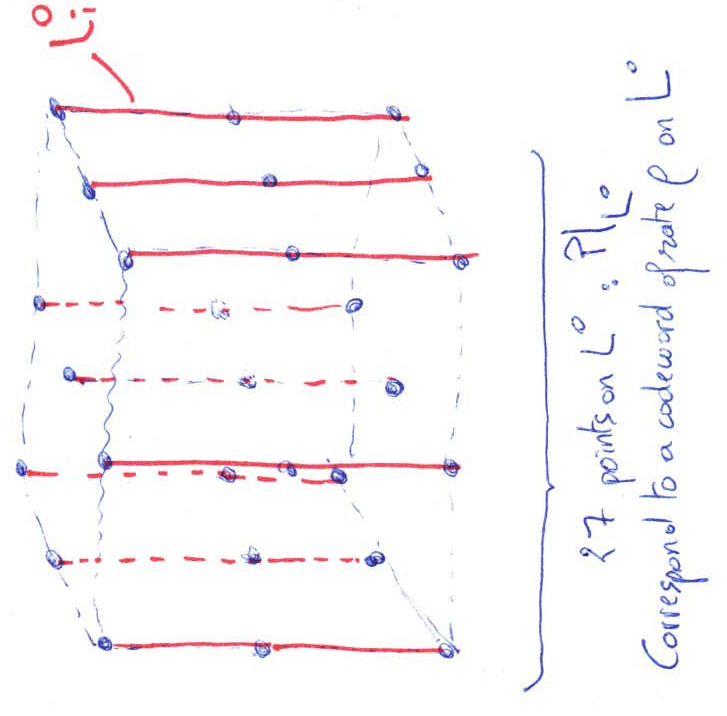
\includegraphics[%
                    angle = 270,
                    origin = c,
                    width = 0.5\textwidth]{fri_1.png}
    \caption{Partition of $L^0$ in copies of ${L^0_i}$}
    \label{fig:my_label}
\end{figure}

\gus{These pictures are awesome! ;-)}
In this example the polynomial is evaluated on the "cube" $L^0$ containing $27$ points. From the partition (the cube is partitioned in 9 vertical red lines, $L^0_i$) we see that $|L^0|=9|L^0_i|$. The idea is to see the evaluation of $P$ on $L^0$ as a tuple of evaluations of $P$ on all the $L^0_i$'s. First the prover commits to the evaluation of $P$ on $L^0$ to obtain the vector $f^0$. On each of the $L^0_i$, the prover computes a polynomial equal to $P$ (not by interpolating, but by using an algebraic procedure described in the next section, which makes directly use of $P$ \gus{Consider explaining this procedure here, and give these 9 polynomials a name.  Aren't these 9 polynomials just $P|_{L^0_i}$?}), of degree $|L^0_i|-1$. So the prover has now $9$ polynomial of degree $|L^0_i|-1$.

\begin{figure}[h!]
    \centering
    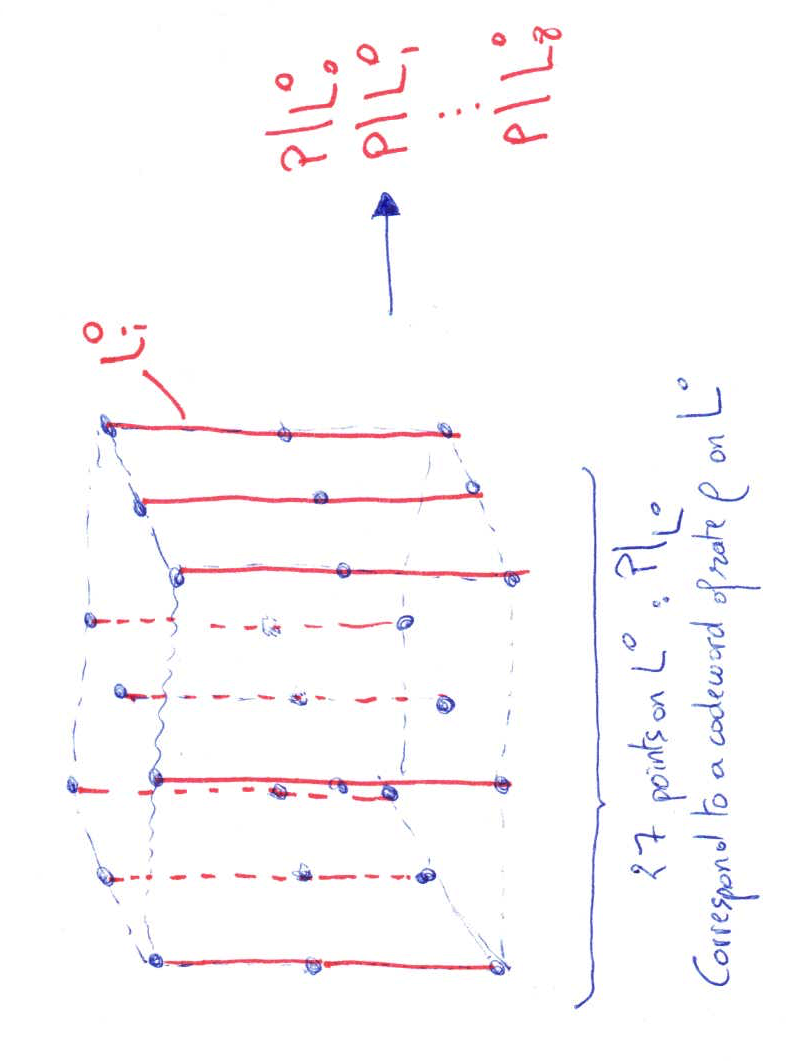
\includegraphics[%
                    angle = 270,
                    origin = c,
                    width = 0.5\textwidth]{fri_2.png}
    \caption{Interpolation of $9$ ($=|L^0|/|L^0_i|$) polynomials of degree $|L^0_i|$ by restricting $P$ on each of the $L^0_i$}
    \label{fig:my_label}
\end{figure}

To construct the next codeword, the prover interacts with the verifier by asking her a random point $x$ in $\mathbf{F}$. The prover will evaluate the $9$ new polynomials $P|_{L^0_i}$ on the point $x$. The prover has now $9$ new points... That form a Reed Solomon code of rate $\rho$, evaluated on a set $L^1$ of size $|L^0|/|L^0_i|$.

\begin{figure}[h!]
    \centering
    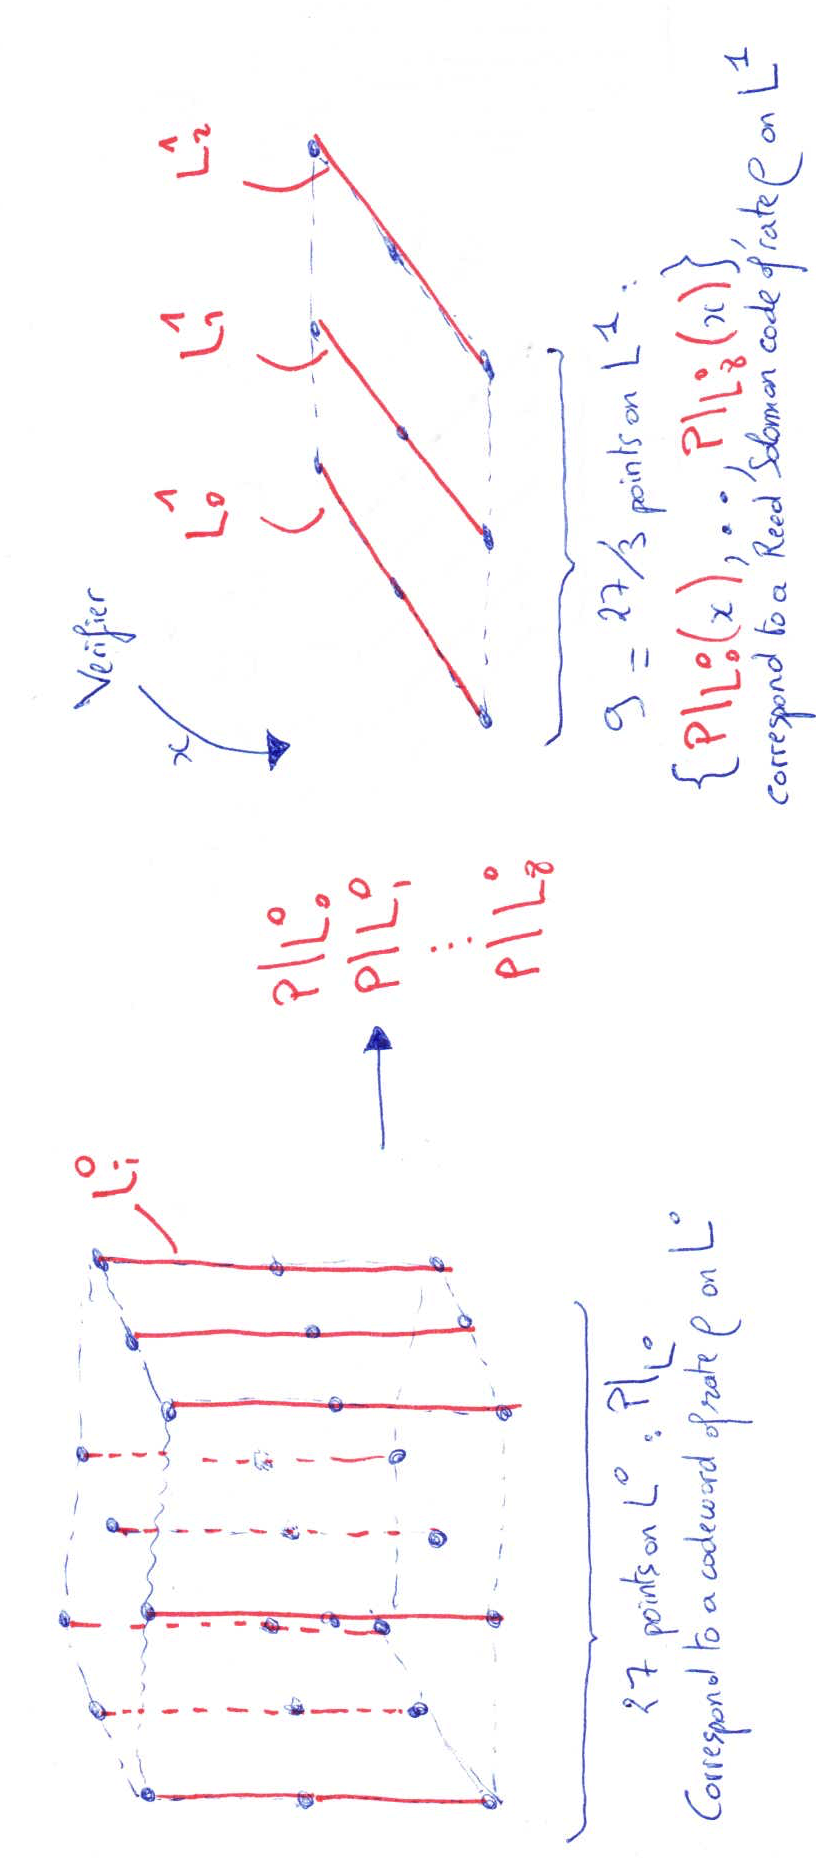
\includegraphics[%
                    angle = 270,
                    origin = c,
                    width = 0.5\textwidth]{fri.png}
    \caption{Creation of a new Reed Solomon codeword using the $9$ polynomials previously created, evaluated on a random point provided by the verifier. Each vertical red line is compressed to yield one point.}
    \label{fig:my_label}
\end{figure}

We can see geometrically why it is still a Reed Solomon code of rate $\rho$, but on $L^1$, with some additional requirements:
\begin{itemize}
    \item The $L^0_i$ are of same size
    \item $L^0$ is a vector space, that can be algebraically described as the zero of a polynomial $Q$
    \item $L^0_0$ is a sub vector space, algebraically described as the zero of a polynomial $Q_0$ with $Q_0|Q$
    \item The $L^0_i$ are cosets of $L^0_0$, algebraically described as the zero of $Q_0-y_i$ for $y_i$ in $L^i$ \gus{Typo?  I don't think you mean $L^i$.  The set $\{y_i\}_i$ is a transversal for $L^0_0$ in $L^0$.  Have you given this set a name yet?}
\end{itemize}
These conditions imply that the $Q_0-y_i$ are pairwise prime (because $L^0_i$ form a partition) and that $Q=\prod (Q_0-y_i)$ (for the same reason). The degree of $Q_0$ then corresponds to the number of points in $L^0_0$.

The initial polynomial $P$ is of degree $<\rho|L^0|$, so when creating the polynomials corresponding to the interpolation of $P$ on $L^0_i$, $P|_{L^0_i}$, the prover creates polynomials of degree $|L^0_i|-1$. And there is a way to retrieve the $P|_{L^0_i}$ from $P$ : the Chinese remainder theorem.
\gus{An obvious way to get $P|_{L^0_i}$ from $P$ is to simply evaluate $P$ on $L^0_i$ and interpolate.  Is your method better than this?  How?}
If we express $P$ mod $Q_0-y_i$ for all $i$, we have a complete description of $P$ on $L^0$. To have "for free" the description of $P$ on $L^0_i$, one can introduce a free variable $Y$ and compute $P$ mod $Q_0(X)-Y$. This way, by replacing  $Y$ by the different $y_i$, we have directly the expression of $P$ on $L^0_i$. But $P(X)=P(X,Q_0(X))=P(X,Y)$ \gus{$P$ is a univariate polynomial.  You've overloaded the symbol $P$.} mod $Q_0(X)-Y$. From this we see that the degree in $Y$ of $P(X,Y)$ mod $Q_0(X)-Y$ must be $<deg(P)/deg(Q_0)<\rho |L^0|/|L^0_0|$. When the prover evaluated the $9$ polynomials $P|_{L^0_i}$ in $x$, she expressed $P|_{L^0_i}$ as $P$ mod $(Q_0(X)-y_i)$ and replaced $X$ by $x$. Otherwise said, she computed $P(X,Y)$ mod $Q_0(X)-Y$, replaced $X$ by $x$ to obtain a single variable polynomial, \textbf{of degree $<\rho|L^0|/|L^0_0|$}, and evaluated this polynomial on each of the $y_i$. Note that there is $|L^0|/|L^0_0|$ such $y_i$ because the $L^0_i$ form a partition of $L^0$! So this is it: the prover goes from a Reed Solomon code of degree $<\rho|L^0|$ to a Reed Solomon code of degree $<\rho|L^0|/|L^0_0|$.
\gus{This paragraph is dense.  You might lose some readers here.}

The procedure is repeated $r$ times, until the obtained Reed Solomon code corresponds to a polynomial of sufficiently low degree. All this is called the COMMIT phase. So let's recap what both we have:
\begin{itemize}
    \item A sequence of spaces $L^0\supset L^1\supset\dots\supset L^r$
    \item A sequence of spaces $(L^i_j)_{i,j}$ where $(L^i_j)_j$ is a partition of $L^i$
    \item A sequence of low degree polynomials $(P^i)$ of decreasing degrees \gus{Need to define $P^i$ above.}
    \item A sequence of challenges $(x_i)$
    \item A sequence of commitments of the evaluation of the $(P^i)$ on $L^i$, where $P^{i+1}$ depends on the challenge $x_i$
\end{itemize}
The first two points are part of the common setup, shared by the prover and the verifier. The third point describes data only known by the prover. The verifier will only have access to the evaluation of these polynomials on $L^i$. We call these evaluations "oracles". From the verifier's point of view, the prover is an oracle from which she can query the evaluation of functions $f^i$, that are (supposedly) low degree polynomials. The last $2$ points are the results of the interactions between the prover and the verifier. Note the meaning of the third points: it means that the $P^i$ are Reed Solomon code, evaluated on the space $L^i$. Let's call the space of the Reed Solomon codes of rate $\rho$ on $L^i$ $RS^i$.

Once this step is finished, the verifying part consists of the following. We have now a sequence of $L^i$, each one partitioned into sets $L^i_j$, where for a given $i$ $(L^i_j)_j$ have same size, as well as a sequence of "challenges" $x_i$ sent by the verifier.

The verifying part (VERIFY) is done like this: the verifier will sample a sequence of $s_i\in L_i$. Each $s_i$ is in one the space $L^i_j$ because they form a partition. The verifier will interpolate the polynomial of degree $|L^i_j|$ corresponding to the evaluation of $P$ on $L^i_j$, $P^j$, and she will evaluate $P^j$ on $x_i$. She will then query from the prover the $i-th$ entry of the Reed Solomon code of step $i$ from the prover: it should match the value $P_j(x_i)$!
\gus{Typo? You have not used the $s_i$ points.  You switched from $s_i$ to $x_i$.}

The sequence $L^i$ stops when the polynomial evaluated on it is of sufficiently low degree for the verifier to make the interpolation directly, and check that the points lie on a degree $<\rho |L^i|$ polynomial.

\section{Algebraic view}

In order to make an algorithm out of the geometric view, we need an algebraic representation of $(L^i)_i$, and of their partition. A super nice thing would be that the $(L^i)_i$ have a group structure: this way to partition them is easy, by just taking a subgroup of it! An even nicer thing would be that the $(L^i)_i$ are in fact linear subpsaces (affine or vector subspaces of the finite field $\mathbf{F}$ on the base field $\mathbf{F}_p$). Why so? Because when the $(L^i)_i$ are affine subspaces there is a super nice way to express them as zeros of a polynomial which has nice properties: $\prod_{a\in L^i}(X-a)$.
\gus{Circular dependency: you are expressing $L^i$ in terms of $L^i$ in the product.}
This polynomial is linear because it's a linear combination of monomials whose degree is a power of $p$, the characteristic of the base field.
\gus{Linear?! This is not clear to me.}

So the idea here is for the prover and the verifier to agree upon a choice of sequence of affine subspaces of decreasing dimensions, $(L^i)_i$, and for each one an affine subspace of low dimension $L^i_0$, and take as a partition the cosets of $L^i_0$ in $L^i$, with $L^i/L^i_0\simeq L^{i+1}$:

\begin{figure}[h!]
    \centering
    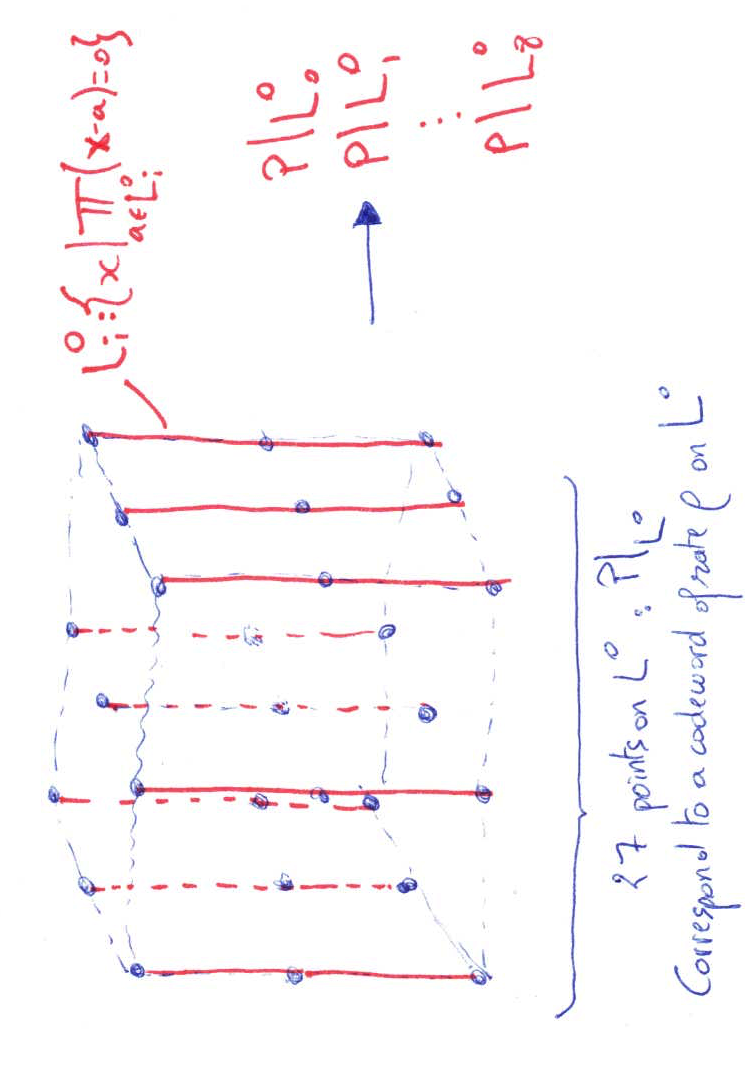
\includegraphics[%
                    angle = 270,
                    origin = c,
                    width = 0.5\textwidth]{fri_algebra_1.png}
    \caption{$L^0_i$ as an affine space, expressed az zeros of a polynomial}
    \label{fig:my_label}
\end{figure}

$L^i_0$ is algebraically described as the zeros of $R_i=\Pi_{a\in L^i_0}(X-a)$. Since this polynomial is in fact a linear application, it also provides a mapping from $L^i$ to $L^{i+1}$, whose kernel is $L^i_0$. Using this, each coset of $L^i_0$ in $L^i$ is mapped to one point on $L^{i+1}$.

Now let's translate algebraically what happens geometrically. Let's call $P$ the initial polynomial of degree $<\rho|L^0|$. The prover commits to the evaluation of this polynomial on $L^0$. The prover then computes $Q(X,Y)=P(X)$ mod $(Y-\Pi_{a\in L^0_0}(X-a)$.
\gus{Now I'm confused.  It seems from this equation that $\prod_{a\in L^0_0}(X-a)$ is just the polynomial $Q_0(X)$ from the previous section.  You said that these polynomials are linear, but I thought the $Q_i(X)$ are non-linear in general.  Indeed, you said in the previous section that $\deg(P)/\deg(Q_0)<\rho|L^0|/|L^0_0|$, implying that $\deg(Q_0)$ must be larger than 1, so that $Q_0$ must be non-linear.}
It is this operation that will keep us dealing with Reed Solomon code words, and that we dubbed "multiple" in the previous section.
\gus{This is the first occurrence of the word ``multiple'' in the paper.}

For example, if $R(X)=X^2$, we see that $P(X)=A(X^2) + X*B(X^2)=A(Y)+X*B(Y)$ mod $(Y-R(X))$. An easy computation shows that the degree of $Q$ in $X$ is $<deg(R)$ and the degree of $Q$ in $Y$ is at most $deg(P)/deg(R)$, \gus{What is $Q$ here?} so in our case, the degree in $Y$ is $<\rho|L^0|/|L^0_0|$, and the degree in $X$ is $<deg(R_0)$. It's exactly what was described in the geometric description.

Now it's clear how the interaction with the verifier will create another Reed Solomon code of the same rate, but on $L^1$: the verifier sends the prover the challenge $x\in\mathbf{F}$, and the prover computes $Q(x,y)$ for all $y\in Im(R_i)$ where $R_i$ is defined on $L^i$.

Note that the polynomial $\prod_{a\in L^i_0}(X-a)$ acts as a compression function. \gus{Earlier you said this polynomial is linear.  It can't be a compression function if it's linear.}  It maps each coset of $L^i_0$ of $L^i$ on one point of the set $L^{i+1}$. So for each point $y\in L^{i+1}$, there is exactly one copy of $L^i_0$ in $L^i$ that is mapped to $y$. We call this particular coset $y_S$.

The following figure illustrates the process:

\begin{figure}[!h]
    \centering
    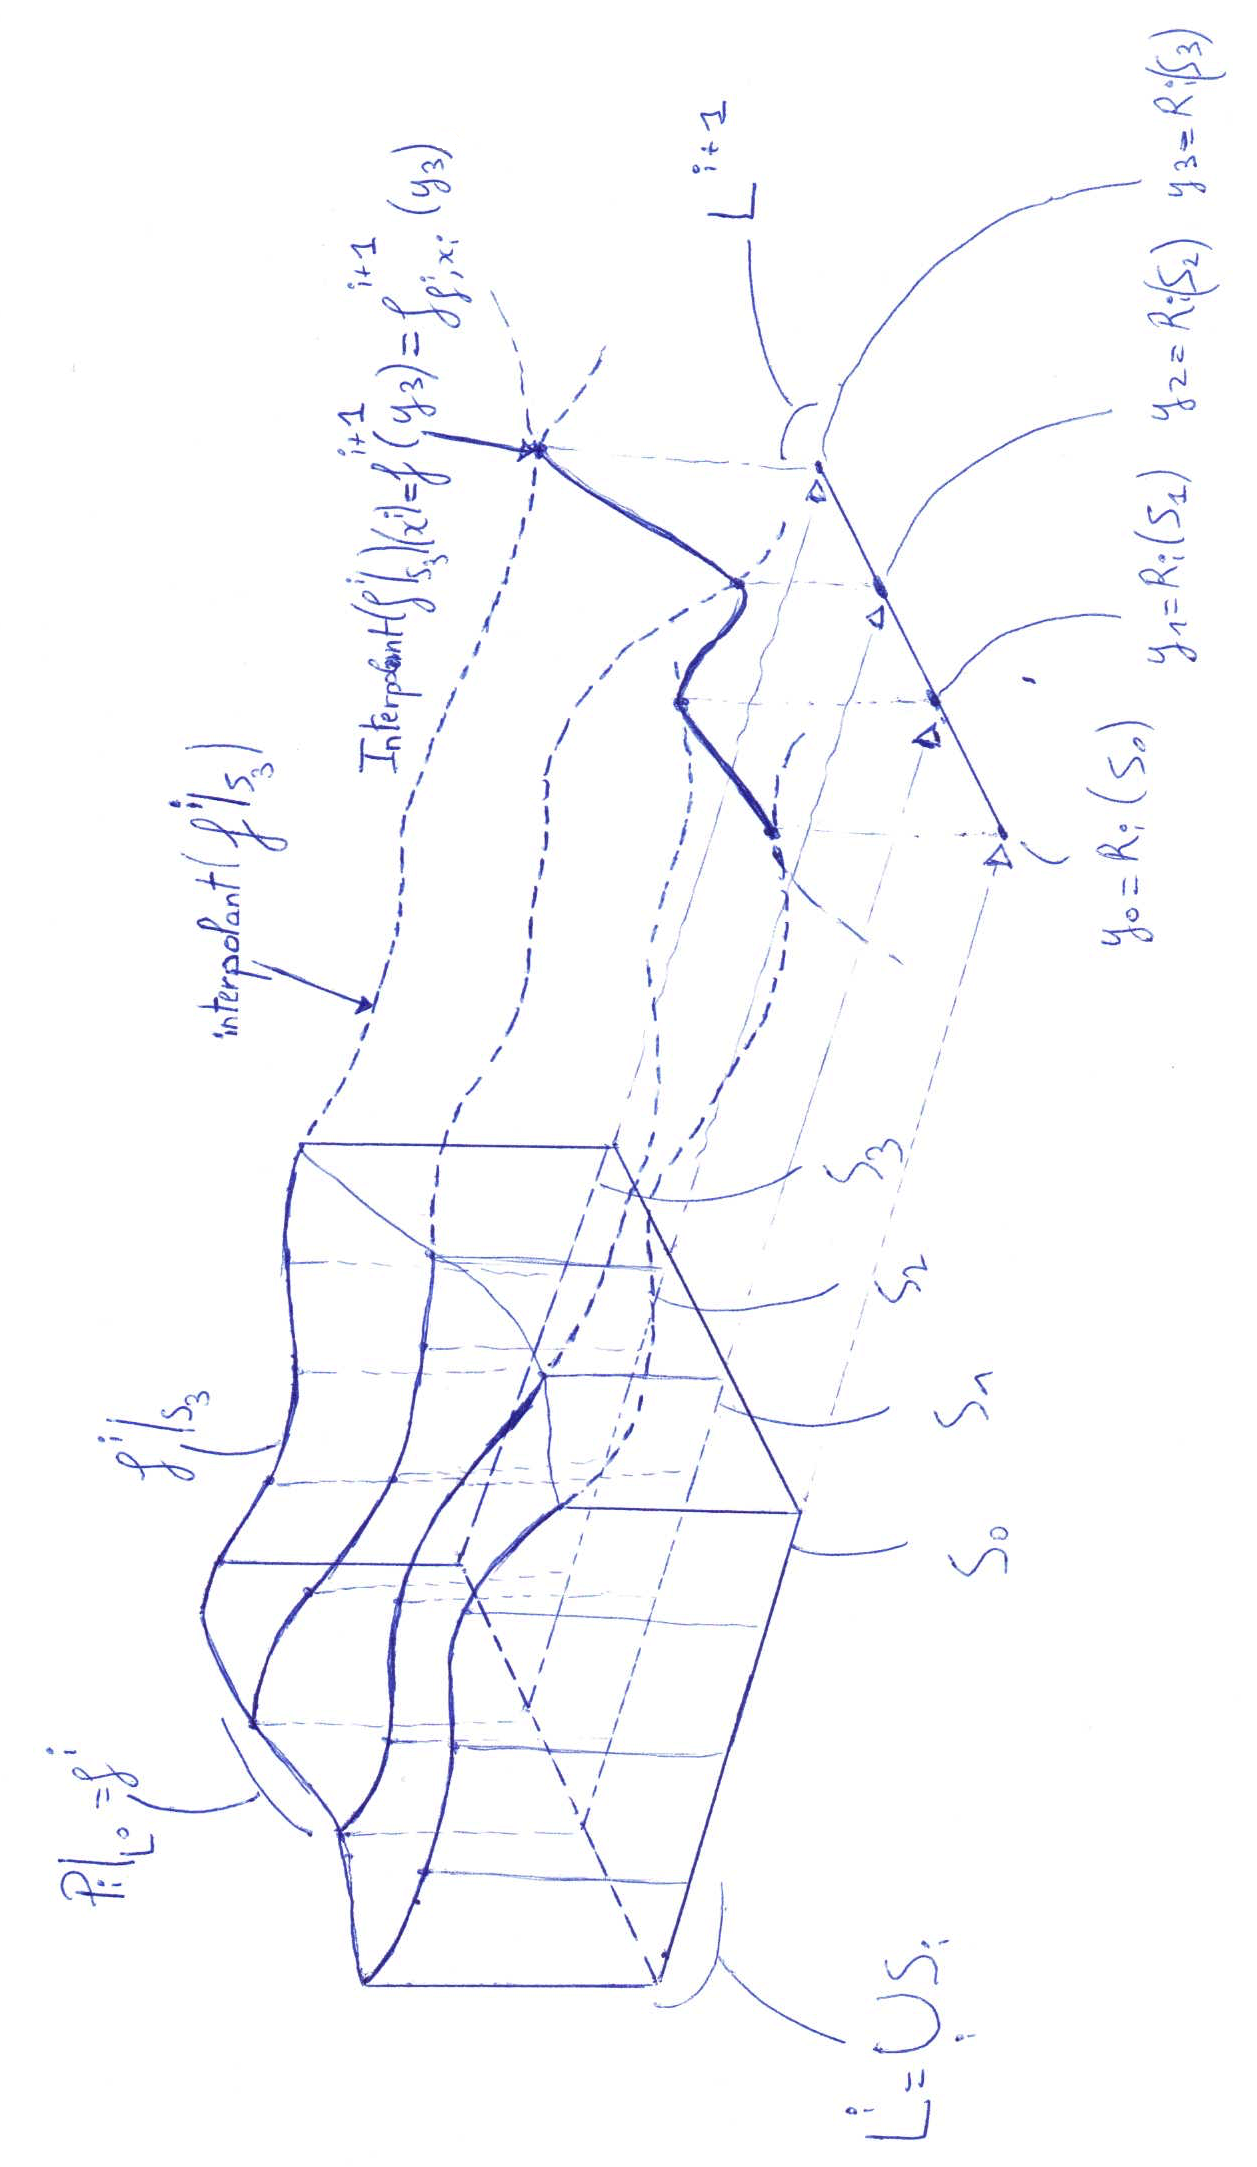
\includegraphics[%
                    angle = 270,
                    origin = c,
                    width = \textwidth]{big_picture.jpg}
    \caption{$L^i$ is the disjoint union of the $(S^i)_i$. On each $S^i$, the verifier interpolates $f^i|_{S_i}$ and evaluate the resulting polynomial at $x^i$. If the prover is honest it should equal $f^{i+1}(y_i)$ where $y_i=R_i(S^i)$.}
\end{figure}

\section{Soundness}

\gus{The primary topic of this post is FRI soundness, but we only begin to talk about soundness on now.  The information in the previous sections is helpful to me, but is all of this information needed before we can talk about soundness?}

Well this algorithm seems nice, but its efficiency has to be assessed now. The natural question is: how strong this algorithm is? That is if the prover cheats during the process (either in the COMMIT phase or the VERIFY part), what are the chances that the VERIFY part outputs YES (meaning the initial commitment indeed corresponds to a Reed Solomon code)?

To answer this let's compute a lower bound of the probability that the VERIFY part outputs NO knowing that the prover cheats, that is that the prover initially has an oracle $f^0$ \textbf{that is not a Reed Solomon code} of rate $\rho$ on $L^0$. Note that there is two ways for the prover to hope the test will pass: first, the prover does the COMMIT step honestly, and pray for the verifier to send challenges that will turn the original non Reed Solomon commitment into a Reed Solomon code. The other way is for the prover to cheat when she provides the oracles to the verifier: at some step, she can modify $f^i$ by not respecting the procedure in the COMMIT step, so that $f^i$ is a Reed Solomon code.

We begin with some definitions that will be useful to understand the process. The purpose of these definitions is to provide a nice set a different distances, to measure the different ways for a set of points to be far from a Reed Solomon code.
\begin{defn}
At step $i$, the space $L^i$ is partionned into subsets $(L^i_j)_j$ of equal size. So a vector $(a_1,\dots,a_{|L^i|})$ can be written as $(A_1,\dots,A_{|L^i|/|L^i_j|})$ where $A_i$ is a vector of size $|L^i_j|$. The smallest number of blocks $A_j$ that you have to correct for the vector $(a_1,\dots,a_{|L^i|})$ to be a Reed Solomon code is called the \textbf{Blockwise distance} from a vector to a Reed Solomon code. We note it $\delta^i$. \gus{Good!}
\end{defn}
The natural distance is the Hamming distance, that we define here.
\begin{defn}
The \textbf{Hamming distance} of the vector $(a_1,\dots,a_{|L^i|})$ to a Reed Solomon code is the smallest number of entries that needs to be changed for the vector to be a Reed Solomon code. We note it $\delta_h^i$.
\end{defn}
Now let's provide a definition that captures the idea that an error occurs during the $i-th$ round of the VERIFY step. Note that this event occurs after the COMMIT step, so it depends on the challenge $x_i$ provided by the verifier.

What this definition really means is that the verifier will sample a point $y\in L^i$ \gus{Typo?  The verifier's challenges were denoted $x$, not $y$.} where the construction of the oracle $f^i$ was wrong. To compute the probability of stumbling upon such a bad $y$, we just divide the number of points of this set by the number of points in $L^i$.

Finally, one last set definition, which will capture the fact that \textbf{during the COMMIT step}, the verifier will provide challenges $x_i$ which will favor the cheating prover, that is the challenges $x_i$ will make the false Reed Solomon code $f^i$ at step $i$ become closer to a real one at step $i+1$.

\begin{defn}
Let $f^{i-1}$ is the oracle at step $i-1$, and $\epsilon>0$. $B(f^{i-1},\epsilon)=\{x\in\mathbf{F}|\delta_h(f_i)<\epsilon\}$ is called the distortion set: it represents the fact that the verifier sent a challenge such that at step $i$ the new oracle created by the prover is closer to a Reed Solomon code than at step $i-1$.
\gus{Actually, it means something stronger.  Not only is it ``closer'' to a RS codeword, it is also \textit{within $\epsilon$ in hamming distance} to a RS codeword.}
\end{defn}
We illustrate what this definition means with some observations on the distances (Hamming vs Blockwise). First, note that the set of different values that can take either of the two distances is \textbf{finite}: indeed $\delta^i_h(f^i)$ is the Hamming distance between $f^i$ and the space of Reed Solomon codes, the smallest unit of distance if $1/|L^i|$ and the different distances possible are multiple of this unit. For the blockwise distance it is the same: $\delta^i(f^i)$ represents the number of cosets in $L^i$ on which $f^i$ differs from the ones in the closest Reed Solomon code. Since the number of cosets is $c_i=|L^i|/|L^i_0|$, the smallest unit that $\delta^i$ can take is $1/c_i$ and the different distances are multiple of this smallest unit. Another useful remark is that the blockwise distance $\delta^{i-1}$ and the Hamming distance $\delta^i_h$ take the same values (i.e. the discretisation is the same). The reason is that each coset in $L^{i-1}$ is mapped to exactly one point on $L^i$. Now what happens if $x\in B(f^{i-1},1/c_{i-1})$?. Well the next oracle is \textbf{strictly} closer to a Reed Solomon code. Since $1/c_{i-1}$ is the smallest unit of distance for the Hamming distance \textbf{at step $i$}, it means that the next oracle \textbf{is} a Reed Solomon code. In the particular case where it happens at the first challenge $x$, the cheating prover is lucky and the VERIFY step will output ACCEPT with probability $1$.

\gus{It seems strange that the FRI authors bothered to define the distortion set as if distance were a continuous quantity.  It seems that discussion could be much simpler by forgetting about distortion sets and just talking about the event that the next polynomial is a RS codeword.}

\begin{figure}[!h]
    \centering
    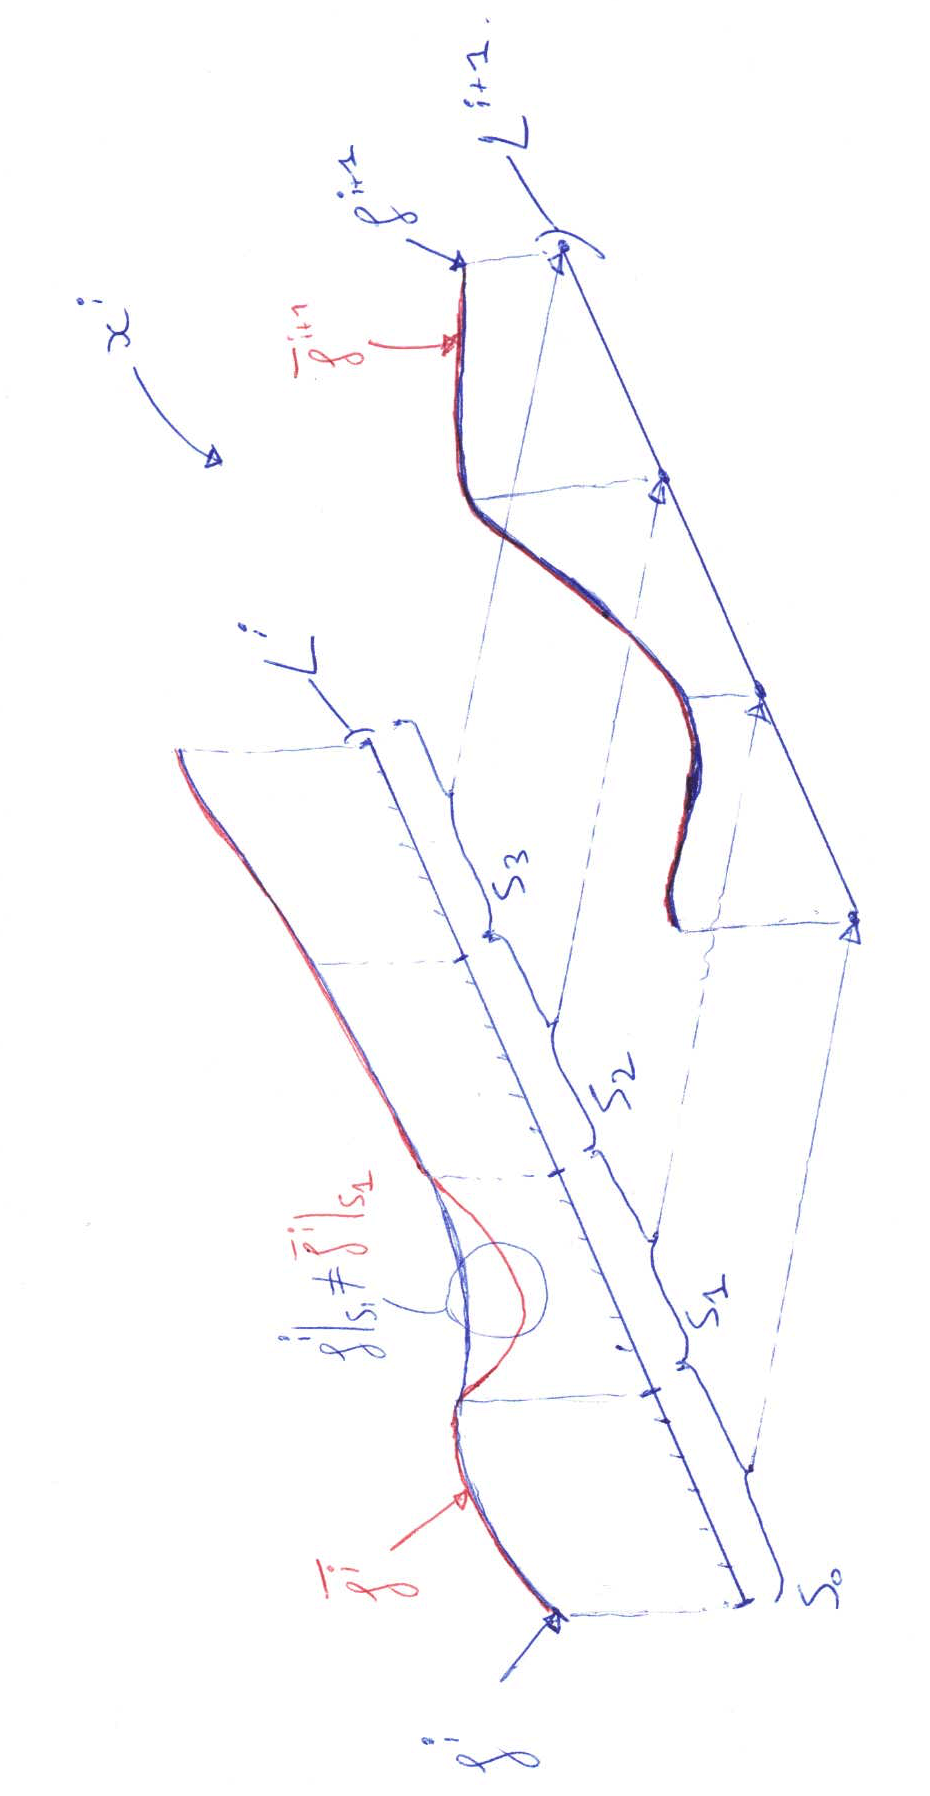
\includegraphics[%
                    angle = 270,
                    origin = c,
                    width = \textwidth]{bad_event.jpg}
    \caption{$\delta^i=1/4$ and $\delta_h^{i+1}<1/4$ so the only possibility is $0$ since the Hamming distance here is a mutliple of $1/4$. So $x^i$ is such that at step $i+1$, $f^{i+1}$ is a Reed Solomon code.}
\end{figure}

So to have a lower bound of the probability of rejection when the first oracle $f^0$ is not a Reed Solomon code, the strategy is the following: first weed out the case of $x\in B(f^i,\delta^i)$ where $\delta^i=1/c_i$ (which means that the first challenge sent by the verifier during the COMMIT step turn $f^1$ into a Reed Solomon code and the VERIFY step will always accept), next we compute the probability of rejection, provided that for no $i$, $x_i\in B(f^i,\delta^i)$.

\textbf{First case}: Upper bound of $x_i\in B(f^0,\delta^i)$ where $\delta^i=1/c_i$. For the oracle $f^i$ we note $\bar{f^i}$ the closest Reed Solomon code (of rate $\rho$). We suppose that $\delta^i<(1-\rho)/2$, which means that there is one and only one Reed Solomon closest to the oracle (there is no tie).
\gus{My understanding of our discussion is that you decided not to consider the case $\delta^i\geq(1-\rho)/2$ in order to simplify the presentation.  If so then you should make this clear at some point in the doc.}
This is because two Reed Solomon code can not be closer than $1-\rho$ Hamming distance wise. Indeed if that were the case, they would be two polynomials that agree on at least one more point than their degree: we know in this case that the polynomials are the same. We note $S^i$ all the cosets in $L^i$ (that is all the copies of $L^i_0$). We note $S_B(f^i)=\cup\{S\in S^i|f^i|_S\neq\bar{f^i}|_S\}$ the set of bad cosets. Those corresponds to the cosets that fail to match the closest Reed Solomon code of $f^i$. We note $D^i=\{y|y\in\cup_{S\in S_{B(f^i)}}S\}$ all the elements belonging to some bad coset. Finally, let's note $X_S=\{x\in\mathbf{F}|interpolant(f^i|_S)(x)=interpolant(\bar{f^i}|_S(x)\}$, the set of possible $x$ sent by the verifier that correct the some \gus{typo} discrepancy at step $i$.
\gus{Elements of $X_S$ correct a discrepancy only if $S\subseteq S_B(f^i)$.  Presumably you only care about $X_S$ for those $S$.}

\begin{figure}[!h]
    \centering
    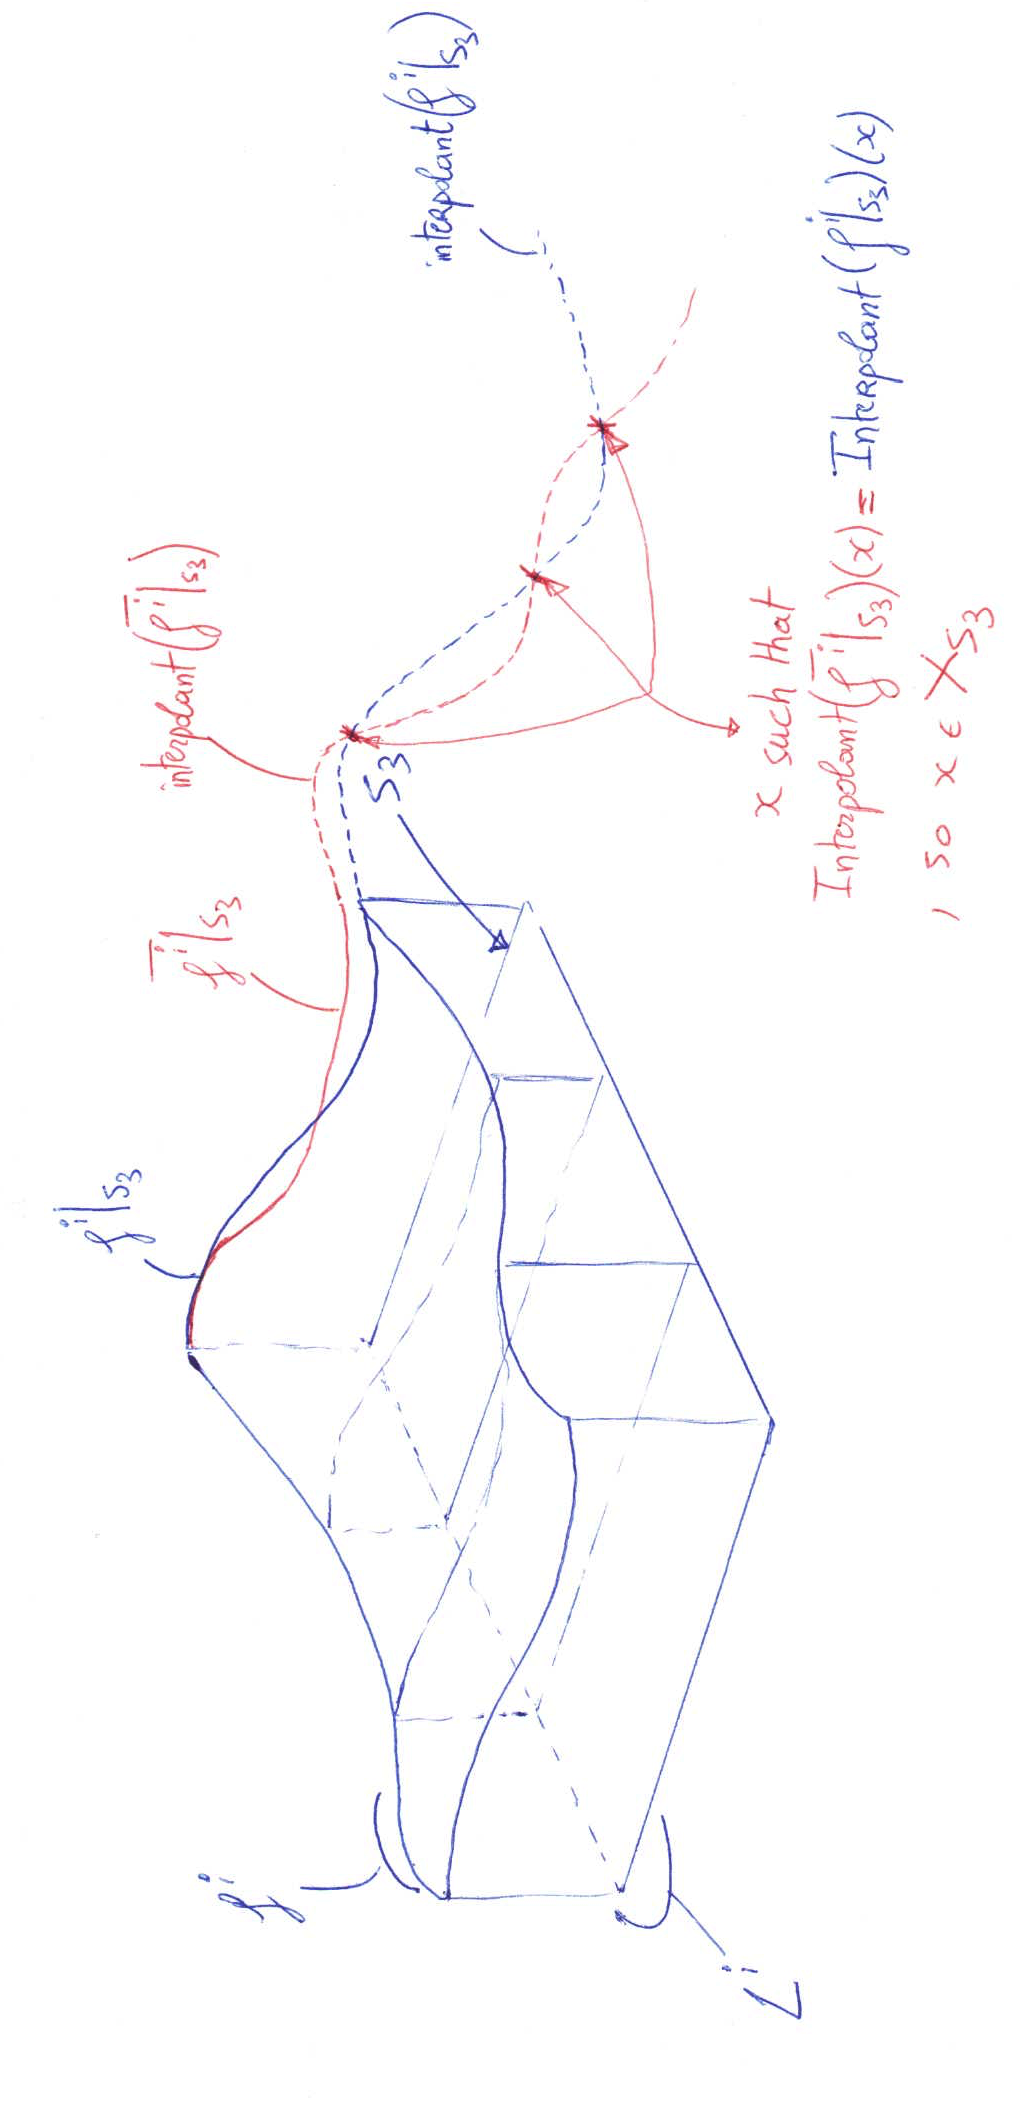
\includegraphics[%
                    angle = 270,
                    origin = c,
                    width = \textwidth]{X_S.jpg}
    \caption{Some $x\in X_{S_3}$: we see that for those $x$, $interpolant(f^i|_{S_3})(x)=interpolant(\bar{f}^i|_{S_3}(x))$.}
\end{figure}

We observe that $B(f^i,\delta^i)=\cup_{S\in S_{B(f^i)}}X_S$ and that $\delta^i=|S_{B(f^i)}|$.
\gus{I'm confused.  I thought you fixed $\delta^i=1/c_i$.  Now you are setting $\delta^i$ to an integer larger than 1.  Typo?}
Choosing a $x$ such that $\delta^{i+1}_h<\delta^i$ means that the $x$ has to be such that on at least one $S\in S_{B(f^i)}$ we have $interpolant(f^i|_S)(x)=interpolant(\bar{f^i}|_S(x)$. Now $interpolant(f^i|_S)$ is of degree $<|S|$. So the maximum number of $x$ verifying $interpolant(f^i|_S)(x)=interpolant(\bar{f^i}|_S(x)$ is $|S|-1$ because of the usual argument that two \textbf{different} polynomials of degree $d$ agree on at most $d$ points. Since we repeat this argument for every $S\in S_{B(f^i)}$, the maximum number of $x$ in $B(f^i,\delta^i)$ is $|S_{B(f^i)}|\times|S|<|L^i|$.
\gus{Shouldn't this be $|S_{B(f^i)}|\times(|S|-1)$?  Why is this quantity smaller than $|L^i|$?}
To have the total probability we divide by the number of elements in $\mathbf{F}$. So we have $P(x\in B(f^i,1/c_i))<|L^i|/|\mathbf{F}|$.

\textbf{Second case}: From now on we suppose that during the COMMIT step, no $x$ is in $B(f^i,\delta^i)$. We will only show what happens in a somewhat simple case, that is a case matching the following conditions:
\begin{itemize}
    \item For all $i\in\{0,\dots,r\}$, $\delta^i<(1-\rho)/2$
    \item For all $i\in\{0,\dots,r\}$, $\bar{f}^{i+1}=f^{i+1}_{\bar{f}^i,x^i}$ \gus{This notation is defined below.}
    \item For all $i\in\{0,\dots,r\}$, $x^i\not\in B(f^i,\delta^i)$
\end{itemize}
where $r$ is the number of rounds. The second condition means that if the prover constructs the next oracle $f^{i+1}$ using the closest Reed Solomon code of the oracle $f^i$, then this constructed oracle is a Reed Solomon code that has the additional property to be the closest Reed Solomon code of the oracle $f^{i+1}$ at step $i+1$.

Suppose that for some $i\in\{0,\dots,r\}$, $s_i\in D^i$. We note $j$ the highest index such that $s^j\in D^j$.
\gus{Typo?  Did you switch $x$ for $s$?}

Now we translate the oracle $f^i$ to $\mathbf{0}$, which is a Reed Solomon code. So we have $\bar{f}^i=\mathbf{0}$, and $\bar{f}^{i+1}=f^{i+1}_{\bar{f^i},x^i}=\mathbf{0}$. We can do this translation because the space of Reed Solomon codes \textbf{is a vector space}.
\gus{Are you assuming WOLOG that the polynomial $f$ is the zero polynomial?!  This assumption follows from the fact that RS codewords are a vector space?}

The last of the $3$ conditions above means that $x^{j}\not\in\cup_{S\in S_{B(f^{j})}}X_S$ so we have $f^{j+1}_{f^j,x^j}(s^{j+1})\neq\mathbb{0}$.
\gus{Typo?  Everywhere you have $\mathbb{0}$ I presume you mean $\mathbf{0}$.}
But the condition on $j$ means that $f^{j+1}(s^{j+1})=\bar{f}^{j+1}(s^{j+1})=\mathbb{0}$. So we have that $f^{j+1}_{f^j,x^j}(s^{j+1})\neq f^{j+1}(s^{j+1})$, which exactly means that the VERIFY step will fail at step $j+1$. \gus{Why?} So the probability of failing the VERIFY step with the $3$ conditions above is \textbf{at least} the probability that $s^0\in D^0$, which is by definition $|D^0|/|L^0|=\delta^0$. Since the VERIFY step is done $l$ times, (that is the verifier will sample $l$ times a random sequence $(s^i)_{i\in\{0,\dots,r\}}$ and perform the rounds verifications), the probability for the VERIFY step to accept is \textbf{at most} $(1-\delta^0)^l$.

One can show that we can always reduce to the case where the $3$ conditions above hold. So when no bad event occurs, the probability of acceptance is at most $(1-\delta^0)^l$.

Let's sum up what we have. If during the COMMIT step, one $x^i\in B(f^i,1/\delta^i)$, the probability of rejecting during the VERIFY step is \textbf{at most} $1$. So the probability of rejection is at least the probability that no such event occurs, which is at least $P_1=1-(\sum_i|L^i|/|\mathbf{F}|)$ from the first point, which means that the probability of acceptance is \textbf{at most} $1-P_1$.

Then when no such event occurs, all that remains for the prover is to cheat during when providing the oracles, so it is the second case we described above. In this case we saw that the probability of acceptance is \textbf{at most} $(1-\delta^0)^l$.

Combining those two cases, we have that the probability of rejection when the first oracle $f^0$ is $\delta^0$ far from a Reed Solomon code (blockwise distance) is \textbf{at least} $1-$(upper bound probability of acceptance) = $1-(1-P_1 + (1-\delta^0)^l)$

\end{document}
